\documentclass{article}
\usepackage{cite}
\usepackage{tabularx}
\usepackage{graphicx} % Required for inserting images
\usepackage{dirtytalk}
\usepackage{pgfplotstable} 
\usepackage{pgfplots}
\usepackage{datatool}
\usepackage{siunitx}
\usepackage[hyphens]{url}  % Allows line breaks at hyphens
\usepackage{hyperref}
\usepackage{graphicx}
\usepackage{microtype}
\usepackage{float}

\hypersetup{
    colorlinks=true,
    linkcolor=blue,
    filecolor=blue,      
    urlcolor=blue,
    citecolor=blue,
}


\title{Assignment 1\\Automated Test Generation Fundamentals}
\author{Casper Kristiansson}
\date{\today}

\begin{document}

\maketitle

\section{Test Creation}

If we want to write test cases that should cover all edges in the control graph which can be seen in figure \ref{fig:graph} we can start by analyzing the possible different paths. The paths can be divided up into:

\begin{itemize}
    \item \textbf{Test Case 1:}
    \begin{itemize}
        \item \textbf{State:} The path list is empty
        \item \textbf{Test Path:} [1, 2, 5]
    \end{itemize}
    \item \textbf{Test Case 2:}
    \begin{itemize}
        \item \textbf{State:} The path list contains one element but does not equal the parameter n.
        \item \textbf{Test Path:} [1, 2, 3, 2, 5]
    \end{itemize}
    \item \textbf{Test Case 3:}
    \begin{itemize}
        \item \textbf{State:} The path list contains more than one element but none equals the parameter n.
        \item \textbf{Test Path:} [1, 2, 3, ..., 2, 5]
    \end{itemize}
    \item \textbf{Test Case 4:}
    \begin{itemize}
        \item \textbf{State:} The path list contains elements and n is found at the first index.
        \item \textbf{Test Path:} [1, 2, 3, 4]
    \end{itemize}
    \item \textbf{Test Case 5:}
    \begin{itemize}
        \item \textbf{State:} The path list contains elements and n exists not at the first index.
        \item \textbf{Test Path:} [1, 2, 3, ..., 3, 4]
    \end{itemize}
\end{itemize}

If the goal is to find possible bugs in the method we can analyze everything that happens in the method. The following inputs are examples of what should be tested to make sure that the method behaves as expected:

\begin{itemize}
    \item Passing null as a parameter to the function
    \item Custom object for the parameter which possibly could have overridden the equals method
\end{itemize}

If the goal is to automatically generate tests for this function one might use a framework such as JUnit. This framework will try to automatically produce tests based on a control flow graph and by creating edge cases for the input. This means by analyzing the control flow graph it can identify possible bugs that might happen.

When trying to mimic a user's behavior it is important to test the main functionality of the function but also actions that might happen like unexpected actions. It might not always be useful to test a wide range of possible edge cases but overall it is important to test and make sure that a function works as expected.

\begin{figure}[H]
    \centering
    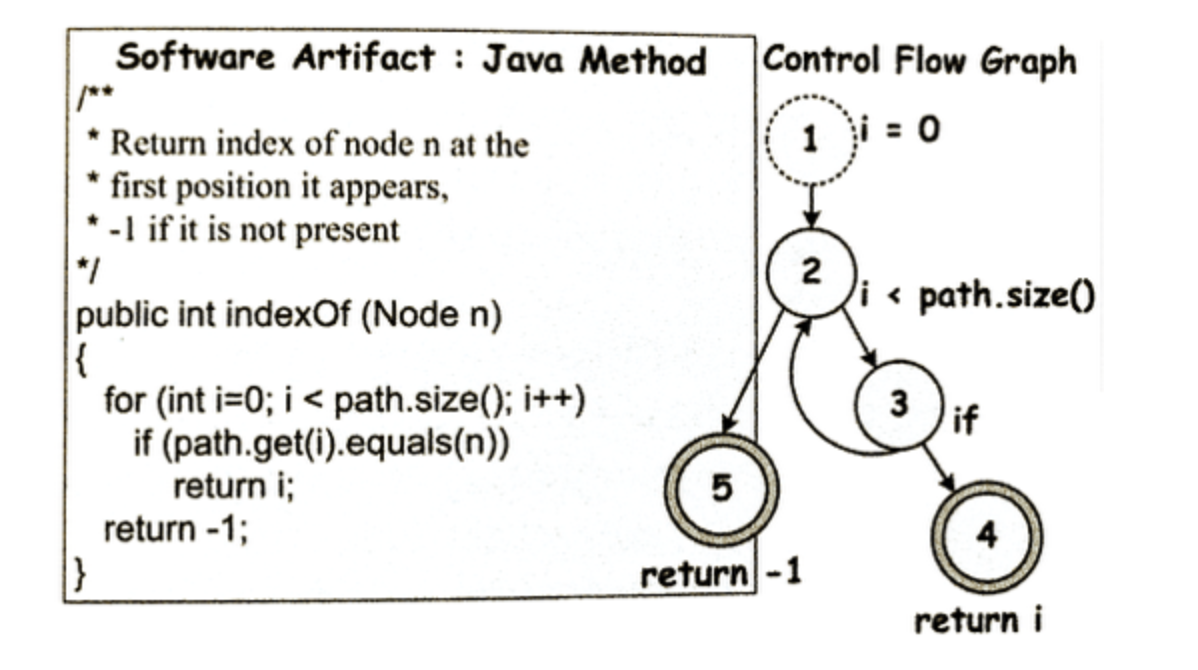
\includegraphics[width=\textwidth]{controlGraph.png}
    \caption{Example Method with Control Graph \cite{Lecture1}}
    \label{fig:graph}
\end{figure}

\section{Taxonomy}
\subsection{Pynguin (Python)}
\begin{enumerate}
    \item \textbf{Software Artifact}
    \begin{enumerate}
        \item \textbf{Implementation}: Source, generatests test based on python source code.
        \item \textbf{Characteristics}: Application/System because it generates tests for Python applications/systems
        \item \textbf{Programming Language}: Python
    \end{enumerate}
    \item \textbf{Implementation}
    \begin{enumerate}
        \item \textbf{Code}: Method level because the testing tools generate unit tests for different methods
        \item \textbf{Monitoring}: Dynamic, because it executes the code and than monitor its behaviour
    \end{enumerate}
    \item \textbf{Test Generation}
    \begin{enumerate}
        \item \textbf{Objective}: Code coverage, \say{...aims to automatically generate unit tests that maximise code coverage.} \cite{lukasczyk2020automated}.
        \item \textbf{Technology}: Search-Based Testing, Chapter 3 \cite{lukasczyk2020automated}.
    \end{enumerate}
    \item \textbf{Test Execution}
    \begin{enumerate}
        \item \textbf{Online/Offline}: Offline
    \end{enumerate}
    \item \textbf{Test Oracle}
    \begin{enumerate}
        \item \textbf{Categories}: Manual, \say{So far, Pynguin focuses on test-input generation and excludes the generation of oracles.} \cite{lukasczyk2020automated}.
    \end{enumerate}
\end{enumerate}

\subsection{Randoop (Java)}
\begin{enumerate}
    \item \textbf{Software Artifact}
    \begin{enumerate}
        \item \textbf{Implementation}: Source, generates tests from Java source code.
        \item \textbf{Characteristics}: Application/System because it generates tests for Java applications/systems
        \item \textbf{Programming Language}: Java
    \end{enumerate}
    \item \textbf{Implementation}
    \begin{enumerate}
        \item \textbf{Code}: Method level because the testing tools generate unit tests for different methods
        \item \textbf{Monitoring}: Dynamic, Randoop uses sequences \say{Each call in the sequence includes a method name and input arguments...} \cite{pacheco2007feedback} to observe the execution of code to generate tests.
    \end{enumerate}
    \item \textbf{Test Generation}
    \begin{enumerate}
        \item \textbf{Objective}: Code coverage
        \item \textbf{Technology}: Random, \say{Our technique builds inputs incrementally by randomly selecting a method call...} \cite{pacheco2007feedback}.
    \end{enumerate}
    \item \textbf{Test Execution}
    \begin{enumerate}
        \item \textbf{Online/Offline}: Offline
    \end{enumerate}
    \item \textbf{Test Oracle}
    \begin{enumerate}
        \item \textbf{Categories}: implicit (observer), \say{RANDOOP can optionally create a regression oracle for each input, ... RANDOOP guesses observer methods...} \cite{pacheco2007feedback}
    \end{enumerate}
\end{enumerate}

\hspace{0cm}
\newpage

\bibliographystyle{IEEEtran}
\bibliography{main}

\end{document}